%\section{Chemistry and Cooling Methods} \label{sec:physics}


% ========== Primoridal Chemistry =========

\section{Primordial Chemistry} \label{sec:primordial_chemistry}
The treatment of primordial chemistry (i.e.\ the chemistry of metal-free gas) used in \texttt{Grackle} is closely based on the
treatment in the Enzo AMR code \citep{2014ApJS..211...19B}, although \texttt{Grackle} accounts for a few processes that are not included 
in the latest version of Enzo available at the time of writing (version 2.5). The Enzo primordial chemistry itself is based 
originally on the work of \citet{1997NewA....2..181A} and \citet{1997NewA....2..209A}, although the current version has been
modified substantially compared to the original Abel~et~al.\ network. In this section, we describe in detail the chemistry 
included in \texttt{Grackle} and discuss how the resulting set of chemical rate equations is solved. 

\subsection{Chemistry Network} \label{sec:network}
\texttt{Grackle} provides three different primordial chemistry networks, differing in the number of chemical species that they include. 
The choice of chemical network is controlled by the \texttt{primordial\_chemistry} parameter. Setting \texttt{primordial\_chemistry = 1} selects the
six species network, which tracks the abundances of the species H, H$^{+}$, He, He$^{+}$, He$^{++}$ and e$^{-}$ and is 
designed for modelling atomic and/or ionized gas. Setting \texttt{primordial\_chemistry = 2} selects the nine species network. This
includes all of the species and reactions included in the six species network, but adds molecular hydrogen (H$_2$), plus the
two ions primarily responsible for its formation in primordial gas (H$^{-}$ and H$_{2}^{+}$). Finally, setting \texttt{primordial\_chemistry = 3}
selects the twelve species network, which is an extension of the nine species model that includes D, D$^{+}$ and HD.

\begin{table}
\caption{Chemical reactions in the six species network \label{tab:six}}
\begin{tabular}{lclcc}
\hline
\multicolumn{3}{c}{Reaction} & \multicolumn{2}{c}{Reference} \\
& & & Data & Fit \\
\hline
${\rm H + e^{-}}$ & $\rightarrow$ & $\rm{H^{+} + e^{-} + e^{-}}$ & 1 & 2 \\
${\rm H^{+} + e^{-}}$ & $\rightarrow$ & $\rm{H + \gamma} $ & 3 & 2, 4\\
${\rm He + e^{-}}$ & $\rightarrow$ & ${\rm He^{+} + e^{-} + e^{-}}$ & 1 & 2 \\
${\rm He^{+} + e^{-}}$ & $\rightarrow$ & ${\rm He + \gamma}$ & 5, 6 & 4, 6, 7 \\
${\rm He^{+} + e^{-}}$ & $\rightarrow$ & ${\rm He^{++} + e^{-} + e^{-}}$ & 1 & 2 \\
${\rm He^{++} + e^{-}}$ & $\rightarrow$ & ${\rm He^{+} + \gamma}$ & 3, 8 & 4, 9 \\
${\rm H + H}$ & $\rightarrow$ & ${\rm H^{+} + e^{-} + H}$ & 10 & 11 \\
${\rm H + He}$ & $\rightarrow$ & ${\rm H^{+} + e^{-} + He}$ & 12 & 11 \\
${\rm H + \gamma}$ & $\rightarrow$ & ${\rm H^{+} + e^{-}}$ & 13 & --- \\
${\rm He + \gamma}$ & $\rightarrow$ & ${\rm He^{+} + e^{-}}$ & 13 & --- \\
${\rm He^{+} + \gamma}$ & $\rightarrow$ & ${\rm He^{++} + e^{-}}$ & 13 & --- \\
\hline
\end{tabular}
\\ Key: 1 -- \citet{1987ephh.book.....J}; 2 -- \citet{1997NewA....2..181A}; 3 -- \citet{1992ApJ...387...95F}; 4 -- \citet{1997MNRAS.292...27H}; 5 -- \citet{1960MNRAS.121..471B}; 6 -- \citet{1973A&A....25..137A}; 7 -- \citet{1981MNRAS.197..553B}; 8 -- \citet{1978ppim.book.....S}; 9 -- \citet{1992ApJS...78..341C}; 10 -- \citet{1987PhRvA..36.3100G}; 11 -- \citet{1991ApJS...76..759L}; 12 -- \citet{1981JChPh..74..314V}; 13 -- see Section~\ref{section:radback}
\end{table}

The reactions included in the six species network are listed in Table~\ref{tab:six}. The rate coefficients for these reactions are implemented in
\texttt{Grackle} using simple temperature-dependent analytical fits. In the Table, we list the references from which we take these fits, and also the 
references that are the original sources of the theoretical or experimental  data on which these fits are based.

A few of the reactions listed in Table~\ref{tab:six} deserve further comment:
\begin{enumerate}
\item[(i)] By default, the recombination of
H$^{+}$, He$^{+}$ and He$^{++}$ is modelled using the case A
recombination rate coefficients (the optically-thin approximation in
which recombination photons above 1 Ryd escape). However, the case B
rate coefficients (in which recombination photons above 1 Ryd are
locally re-absorbed) can instead be selected by setting \texttt{CaseBRecombination} = 1. The additional complication that photons from the recombination of
He$^{+}$ can bring about the photoionization of hydrogen \citep[discussed in some detail in][]{1989agna.book.....O} is not accounted
for, but in most circumstances this will only lead to a small error in the H$^{+}$ and He$^{+}$ abundances. 
\item[(ii)] The rates of the photoionization reactions are not calculated internally by \texttt{Grackle}, but instead are specified either via an input data file or 
passed directly to \texttt{Grackle}  via the  \texttt{Grackle} API as described in Section~\ref{section:radback}.
\item[(iii)] The six species network implemented in \texttt{Grackle} includes two additional reactions that were not part of the original \citet{1997NewA....2..181A}
six species network: the collisional ionization of H by collisions with H and He atoms. Often, these reactions are unimportant. However, they 
can become competitive with the collisional ionization of H by electrons if the fractional ionization of the gas is very low \citep[see, e.g.][for an example of when this can be important]{2015MNRAS.451.2082G}.
\end{enumerate}

\begin{table}
\caption{Chemical reactions in the nine species network \label{tab:nine}}
\begin{tabular}{lclcc}
\hline
\multicolumn{3}{c}{Reaction} & \multicolumn{2}{c}{Reference} \\
& & & Data & Fit \\
\hline
${\rm H + e^{-}}$ & $\rightarrow$ & ${\rm H^{-} + \gamma}$ & 1 & 2 \\
${\rm H^{-} + H}$ & $\rightarrow$ & ${\rm H_{2} + e^{-}}$ & 3 & 3 \\
${\rm H + H^{+}}$ & $\rightarrow$ & ${\rm H_{2}^{+} + \gamma}$ & 4 & 5 \\
${\rm H_{2}^{+} + H}$ & $\rightarrow$ & ${\rm H_{2} + H^{+}}$ & 6 & 6 \\
${\rm H_{2} + H^{+}}$ & $\rightarrow$ & ${\rm H_{2}^{+} + H}$ & 7 & 8 \\
${\rm H_{2} + e^{-}}$ & $\rightarrow$ & ${\rm H + H + e^{-}}$ & 9 & 9 \\
${\rm H_{2} + H}$ & $\rightarrow$ & ${\rm H + H + H}$ & 10 & 10 \\
${\rm H^{-} + e^{-}}$ & $\rightarrow$ & ${\rm H + e^{-} + e^{-}}$ & 11 & 12 \\
${\rm H^{-} + H}$ & $\rightarrow$ & ${\rm H + e^{-} + H}$ & 11 & 12 \\
${\rm H^{-} + H^{+}}$ & $\rightarrow$ & ${\rm H + H}$ & 13 & 14 \\
${\rm H^{-} + H^{+}}$ & $\rightarrow$ & ${\rm H_{2}^{+} + e^{-}}$ & 15 & 12, 16 \\
${\rm H_{2}^{+} + e^{-}}$ & $\rightarrow$ & ${\rm H + H}$ & 17 & 12 \\
${\rm H_{2}^{+} + H^{-}}$ & $\rightarrow$ & ${\rm H_{2} + H}$ & 18 & 18 \\ 
${\rm H + H + H}$ & $\rightarrow$ & ${\rm H_{2} + H}$ & 19  & 19  \\
${\rm H + H + H_{2}}$ & $\rightarrow$ & ${\rm H_{2} + H_{2}}$ & 20, 21 & 22 \\
${\rm H^{-} + \gamma}$ & $\rightarrow$ & ${\rm H + e^{-}}$ & 23 & --- \\
${\rm H_{2}^{+} + \gamma}$ & $\rightarrow$ & ${\rm H + H^{+}}$ & 23 & --- \\
${\rm H_{2} + \gamma}$ & $\rightarrow$ & ${\rm H_{2}^{+} + e^{-}}$ & 23 & --- \\
${\rm H_{2}^{+} + \gamma}$ & $\rightarrow$ & ${\rm H^{+} + H^{+} + e^{-}}$ & 23 & --- \\
${\rm H_{2} + \gamma}$ & $\rightarrow$ & ${\rm H + H}$ & 23 & --- \\
${\rm H + H + grain}$ & $\rightarrow$ & ${\rm H_{2} + grain}$ & --- & 24$^{*}$ \\
\hline
\end{tabular}
\\ Note: the nine species network also includes all of the reactions listed in Table~\ref{tab:six}.
\\ Key: 1 -- \citet{1979MNRAS.187P..59W}; 2 --
\citet{1998ApJ...509....1S}; 3 -- \citet{2010Sci...329...69K}; 4 --
\citet{1976PhRvA..13...58R}; 5 -- \citet{2015MNRAS.446.3163L}; 6 --
\citet{1979JChPh..70.2877K}; 7 -- \citet{2002PhRvA..66d2717K}; 8 ---
\citet{2004ApJ...606L.167S,2004ApJ...607L.147S}; 9 --
\citet{2002PPCF...44.1263T}; 10 -- \citet{1996ApJ...461..265M}; 11 --
\citet{1987ephh.book.....J}; 12 -- \citet{1997NewA....2..181A}; 13 --
\citet{1986JPhB...19L..31F}; 14 -- \citet{1999MNRAS.304..327C}; 15 --
\citet{1978JPhB...11L.671P}; 16 -- \citet{1987ApJ...318...32S}; 17 --
\citet{1994ApJ...424..983S}; 18 -- \citet{1987IAUS..120..109D}; 19 --
See text; 20 -- \citet{1962JChPh..36.2923S}; 21 --
\citet{1970JChPh..53.4395H}; 22 -- \citet{1983JPCRD..12..531C}; 23 --
see Section~\ref{section:radback}; 24 -- \citet{1985ApJ...291..722T,
  2000ApJ...534..809O}; * - This reaction included as an additional
option when metals are present.
\end{table}

The nine species network includes all of the reactions in Table~\ref{tab:six} plus the additional reactions listed in Table~\ref{tab:nine}. Again,
a couple of reactions deserve further discussion:
\begin{enumerate}
\item[(i)] The treatment of H$_{2}$ collisional dissociation by H atom collisions now used in \texttt{Grackle} is taken from \citet{1996ApJ...461..265M} and 
accounts for both the temperature and the density dependence of this process. It therefore remains valid in the high density limit, where the H$_{2}$
level populations approach their local thermodynamical equilibrium (LTE) values. This is important, because H$_{2}$ is far more susceptible to
collisional dissociation in this limit than when it is solely in the vibrational ground state. It should also be noted that the treatment of this process
in \texttt{Grackle} accounts for effects of dissociative tunneling as well as direct collisional dissociation; previously, Enzo only accounted for the latter
process and hence underestimated the dissociation rate at low temperatures \citep{2014MNRAS.443.1979L,2015MNRAS.451.2082G}
\item[(ii)] In view of the considerable uncertainty in the rate of the three-body reaction
\begin{equation}
{\rm H + H + H} \rightarrow {\rm H_{2} + H},
\end{equation}
discussed in detail in \citet{2008AIPC..990...25G} and \citet{2011ApJ...726...55T}, \texttt{Grackle} provides several different rate coefficients for this process. The user can
select which of these rate coefficients to adopt by means of the \texttt{three\_body\_rate} parameter. The options are
\begin{enumerate}
\item[{\bf 0}:]  Rate coefficient from \citet{2002Sci...295...93A}, based on an extrapolation from low temperature calculations by \citet{1987JChPh..87..314O}. This is the default option.
\item[{\bf 1}:]  Rate coefficient from \citet{1983ApJ...271..632P}, derived using detailed balance applied to the H$_{2}$ collisional dissociation rate measured by \citet{1967JChPh..47...54J}.
\item[{\bf 2}:]  Rate coefficient recommended by \citet{1983JPCRD..12..531C}, based on a survey of the experimental data available at that time. 
\item[{\bf 3}:]  Rate coefficient from \citet{2007MNRAS.377..705F}, also derived from \citet{1967JChPh..47...54J} using detailed balance, but with a different treatment of the H$_{2}$ partition
function. 
\item[{\bf 4}:]  Rate coefficient from \citet{2008AIPC..990...25G}, derived from the \citet{1996ApJ...461..265M} high-density H$_2$ collisional dissociation rate using detailed balance
\item[{\bf 5}:]  Rate coefficient computed directly by \citet{2013ApJ...773L..25F}.
\end{enumerate}
\end{enumerate}
We plot each of these rates in Figure \ref{fig:threebody}.

\begin{figure}
  \centering
  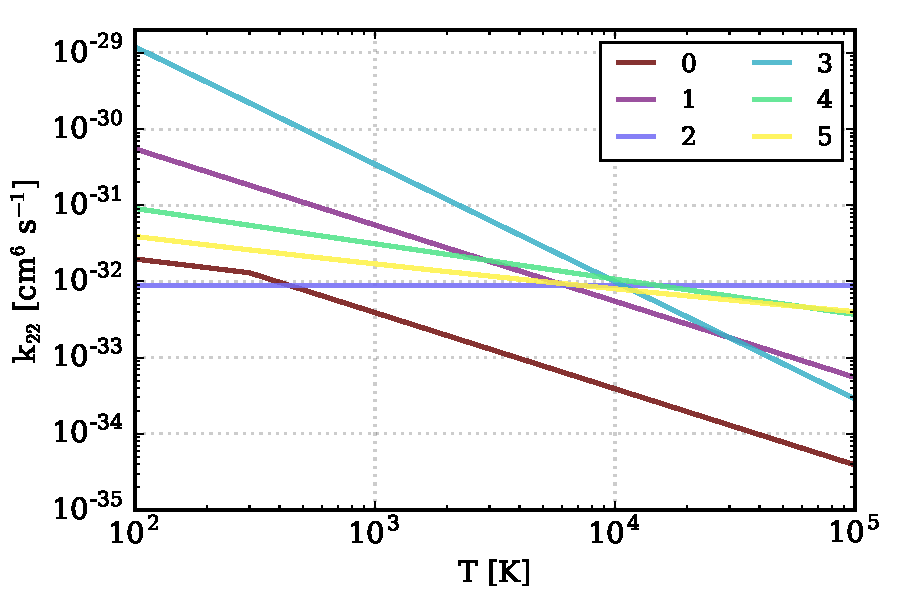
\includegraphics[width=0.45\textwidth]{threebody.pdf}
  \caption{ The available three-body H$_{2}$ formation rates as a
    function of temperature: 0 - \citet{2002Sci...295...93A}, 1 -
    \citet{1983ApJ...271..632P}, 2 - \citet{1983JPCRD..12..531C}, 3 -
    \citet{2007MNRAS.377..705F}, 4 - \citet{2008AIPC..990...25G}, 5 -
    \citet{2013ApJ...773L..25F}.} \label{fig:threebody}
\end{figure}


Finally, the twelve species network includes the reactions in Tables~\ref{tab:six} and \ref{tab:nine}, plus a small number of additional reactions involving
D$^{+}$, D and HD, listed in Table~\ref{tab:12}. The intent of the twelve species network is to allow the HD abundance of the gas to be tracked accurately,
since in cold gas HD can become a more effective coolant than H$_{2}$ despite its much lower fractional abundance \citep[see e.g.][]{2006MNRAS.366..247J,2008ApJ...685....8M}. It is therefore necessary to include only a small number of reactions, as the direct conversion of H$_{2}$ to HD by collisions with D$^{+}$ and D, together with the
corresponding inverse reactions generally dominate the production and destruction of HD.

Two reactions in the twelve species network require further discussion:
\begin{enumerate}
\item[(i)] The rate coefficient that we adopt for the reaction
\begin{equation}
{\rm HD + H} \rightarrow {\rm H_{2} + D}
\end{equation}
is an analytical fit presented in \citet{2002P&SS...50.1197G}, based on data from \citet{1959JChPh..31.1359S}. However, this fit blows up
at temperatures $T < 100$~K, yielding an unphysically large value for the rate coefficient. We therefore follow \citet{2007MNRAS.376..709R}
and \citet{2008ApJ...685....8M} and assume that the rate at $T < 100$~K is the same as the rate at $T = 100$~K. Note that as this reaction
proceeds extremely slowly at temperatures below a few hundred K, this is unlikely to be a significant source of error. 
\item[(ii)] We assume that the rate coefficient for the associative detachment of H$^{-}$ by D
\begin{equation}
{\rm D + H^{-} \rightarrow  HD + e^{-}}
\end{equation}
is the same as for the corresponding reaction between H and H$^{-}$, since measurements by \citet{2012PhRvA..86c2714M} suggest that
there is not a significant isotope effect for this reaction. However, in the solver, we multiply the rate coefficient by a factor of two when
computing the HD formation rate to account approximately for the contribution from the reaction
\begin{equation}
{\rm H + D^{-} \rightarrow  HD + e^{-}}.
\end{equation}
Note that we do not explicitly include this reaction in our network because it would require us to track the abundance of the D$^{-}$ ion,
thereby adding significant additional complexity to the model for only a marginal increase in accuracy.
\end{enumerate}

\begin{table}
\caption{Additional reactions included in the twelve species network \label{tab:12}}
\begin{tabular}{lclcc}
\hline
\multicolumn{3}{c}{Reaction} & \multicolumn{2}{c}{Reference} \\
& & & Data & Fit \\
\hline
${\rm H^{+} + D}$ & $\rightarrow$ & ${\rm H + D^{+}}$ & 1, 2 & 3 \\
${\rm D^{+} + H}$ & $\rightarrow$ & ${\rm D + H^{+}}$ & 1, 2 & 3 \\
${\rm H_{2} + D^{+}}$ & $\rightarrow$ & ${\rm HD + H^{+}}$ & 4 & 5 \\
${\rm HD + H^{+}}$ & $\rightarrow$ & ${\rm H_{2} + D^{+}}$ & 4 & 5 \\
${\rm H_{2} + D}$ & $\rightarrow$ & ${\rm HD + H}$ & 6 & 7 \\
${\rm HD + H}$ & $\rightarrow$ & ${\rm H_{2} + D}$ & 8 & 5, 9 \\
${\rm D + H^{-}}$ & $\rightarrow$ & ${\rm HD + e^{-}}$ & 10, 11 & 10  \\
\hline
\end{tabular}
\\ Note: the twelve species network also includes all of the reactions listed in Tables~\ref{tab:six} \& \ref{tab:nine}.
\\ Key: 1 -- \citet{1999PhRvL..83.4041I}; 2 -- \citet{2000PhRvA..62d2706Z}; 3 -- \citet{2002ApJ...566..599S};
4 -- \citet{1982sasp.nasa..304G}; 5 -- \citet{2002P&SS...50.1197G}; 6 -- \citet{2003PhRvL..91f3201M}; 7 -- \citet{2011ApJ...727..110C}; 
8 -- \citet{1959JChPh..31.1359S}; 9 -- \citet{2007MNRAS.376..709R}; 10 -- \citet{2010Sci...329...69K}; 11 -- \citet{2012PhRvA..86c2714M}
\end{table}

% ----------------------------------

\subsection{Solving and Updating the Network}

Chemical networks such as the ones described above are often challenging to evolve due to the very different time scales that various rates may have -- creation and destruction time scales can differ by orders of magnitude among the different species.   Such ``stiff" sets of equations are often solved with implicit methods, which permit longer timesteps.  Several packages exist to do this, and can even switch between methods for solving stiff and non-stiff equations, such as LSODAR \citep{Hindmarsh83}; however, for multi-dimensional simulations it is useful to have an implementation which is optimized for the case at hand.

Our kinetic network for solving the rate of change of species density $n_i$ has the general form
\begin{equation}
\frac{\partial n_i}{\partial t} = \sum_j \sum_l k_{jl} n_j n_l + \sum_j I_j n_j
\label{eq:rate_general}
\end{equation}
where $k_{jl}$ is the rate for reactions involving species $j$ and $l$ while $I_j$ is the appropriate radiative rate.  Note that in rare cases there may be an additional term for three-body reactions.   To solve this kinetic network, \texttt{Grackle} follows closely the procedure described in \citet{1997NewA....2..209A} and \citet{2014ApJS..211...19B} by grouping creation and destruction rates to rewrite Eq.~\ref{eq:rate_general} as,
\begin{equation}
\frac{\partial n_i}{\partial t} = C_i(T, n_j) - D_i(T, n_j) n_i
\label{eq:rateCD}
\end{equation}
where $C_i$ represents the total creation rate of species $i$ (given the temperature $T$ and other species densities) while $D_i n_i$ is the destruction rate of the same species (which must be proportional to $n_i$), including both radiative and collisional processes.  Ideally, we would solve these ordinary differential equations using a higher order method; however, here we adopt a very simple low order backwards difference formula (BDF) due to its stability.  \citet{1997NewA....2..209A} explored a variety of higher-order solution techniques but found that this simple BDF scheme was generally more stable and competitive for the level of accuracy required.  In particular, the BDF version of Equation~\ref{eq:rateCD} is:
\begin{equation}
n^{t + \Delta t} = \frac{C^{t+\Delta t} \Delta t + n^t}{1 + D^{t+\Delta t} \Delta t}
\label{eq:rate_BDF}
\end{equation}
Unfortunately, we are not able to fully implement a BDF scheme due to
the difficulty of evaluating the $C_i$ and $D_i$ at the advanced time.
Instead, we attempt to mimic a BDF method through a set of partial
updates combined with sub-cycling.  The partial forwarding updating is
done by solving the various species in a specified order and using
the updated species densities in the following partial step.  The
ordering developed by \citet{1997NewA....2..209A} was based on empirical tests under a wide range of conditions and is as follows for the six species model: H, H$^+$, e$^-$, He, He$^+$, He$^{++}$.  For the nine species model, we then add H$_2$, H$^-$, and H$_2^+$.  The H$_2^+$ timescale is sufficiently short that it can be decoupled and we use instead the equilibrium value:
\begin{equation}
n_{ {\rm H}_2^+} = \frac{k_9 n_{\rm H} n_{\rm H^+} + k_{11} n_{\rm H_2} n_{\rm H^+} + k_{17} n_{\rm H^-} n_{\rm H^+} + k_{29} n_{\rm H_2}}
   {k_{10} n_{\rm H} + k_{18} n_{\rm e} + k_{19} n_{\rm H^-} + k_{28} + k_{30}}
\end{equation}
Finally, for twelve species model, we add D, D$^+$ and HD.  In each case, the updated species of the previous step are used in the next.  

The time step passed to \texttt{Grackle} (often the hydrodynamic timestep of a parent simulation) can be quite large, which may potentially cause large errors in our low-order chemical integrator.  To get around this issue, we sub-cycle the BDF step described above, constraining the chemical timestep such that the H and e$^-$ abundances change by no more than 10\% in any sub-cycle step of length $\Delta t$:
\begin{equation}
\Delta t = 0.1 \min \left( \frac{n_{\rm H}}{\dot{n}_{\rm H}} , \frac{n_{\rm e^-}}{\dot{n}_{\rm e^-}} \right)
\end{equation}
In some cases, particularly close to equilibrium, we slightly modify this.  After more than 50 subcycle steps (if we have not yet integrated a full hydro timestep), we replace the analytically calculated time derivatives in the above expression with numerical time derivatives (i.e. change from the previous sub-cycle step).  This is helpful when we are close to equilibrium and the integrator is taking very small steps and regularly overshooting the equilibrium value.  
%Finally, when the density is high $n_H > 10^8$ cm$^{-3}$, and the net cooling/heating term is positive (see below), we replace use an estimate of the rate of change of H based on the H equilibrium solution.

% ============ Cooling/Heating =============

\section{Heating and Cooling} \label{Cooling}

\texttt{Grackle} can evolve the Lagrangian energy equation, taking into account a wide range of radiative cooling and heating processes:
\begin{equation}
\frac{de}{dt} = - \dot{e}_{\rm cool} + \dot{e}_{\rm heat}
\end{equation}
In this paper, we split our discussion of radiative cooling/heating and chemistry, but in the code, they are solved together, using a simple first-order integrator.  To enhance accuracy, the integrator is sub-cycled with a timestep constraint 
\begin{equation}
\Delta t \leq 0.1 \frac{e}{\dot{e}}.
\end{equation}
If both chemistry and cooling/heating are turned on, these are integrated at the same time, using a timestep which is a minimum of the chemistry and cooling constraints.  In the following sections, we describe the various supported cooling and heating options.  We begin with radiative cooling and heating due solely to hydrogen and helium, and then turn to heavier atomic elements (``metals"), and finally dust. 

% ----------------------------------

\subsection{Primordial Heating and Cooling}

To solve for the effects of primordial (H and He only) heating and cooling, \texttt{Grackle} includes two options: (1) a non-equilibrium solver, the chemistry part of which is described in detail in Section~\ref{sec:primordial_chemistry}, and (2) a tabulated version, which assumes ionization equilibrium to compute the cooling and heating rates due to primordial chemistry.  In both cases, photo-heating from an external radiation source can be important -- this is described in Section~\ref{section:radback}.

\subsubsection{Non-equilibrium} \label{sec:pri-neq}

We include a variety of cooling rates due to transitions of the non-equilibrium species.  We begin with a list appropriate for the six species network (\texttt{primordial\_chemistry = 1}): 

\begin{enumerate}
\item Collisional excitation cooling rates involving the following species: $n_{\rm e} n_{\rm H}$, $n_{\rm e}^2 n_{\rm He^+}$, and $n_{\rm e} n_{\rm He^+}$ \citep{1981MNRAS.197..553B, 1992ApJS...78..341C};
\item Collisional ionization cooling for $n_{\rm e} n_{\rm H}$, $n_{\rm e} n_{\rm He}$, $n_{\rm e} n_{\rm He^+}$ and $n_{\rm e}^2 n_{\rm He^+}$ \citep{1987ApJ...318...32S, 1992ApJS...78..341C, 1997NewA....2..181A};
\item Recombination cooling: $n_{\rm e} n_{\rm H^+}$, $n_{\rm e} n_{\rm He^+}$, $n_{\rm e} n_{\rm He^{++}}$ \citep{1981MNRAS.197..553B, 1992ApJ...387...95F, 1997MNRAS.292...27H};
\item Bremsstrahlung cooling for all ionized species \citep{1981MNRAS.197..553B};
\item Compton cooling/heating off the CMB \citep{1971phco.book.....P}, and 
\item Photoionization heating for H, He and He$^+$, depending on the ionizing radiation field -- see section~\ref{section:radback} for more details.
\end{enumerate}
In addition to the sources referenced above, we note that most of these rates were tabulated in Appendix B of \citet{1997NewA....2..209A}.

For the nine species version (\texttt{primordial\_chemistry = 2}), we add H$_2$ cooling.  Our default cooling rate is as follows.  At high densities, where the level populations are in LTE and hence depend only on temperature, we use the high-density rate from \citet{1998A&A...335..403G}. For low densities, we computed the cooling rate due to collisions with H, H$_2$, He, H$^+$, and e$^-$ as described in section 2.3 of  \citet{2008MNRAS.388.1627G}.  The exception is that for collisions with e$^-$, we use revised rates from \citet{yoon2008cross} and for H$^+$, we adopt rates from \citet{2011PhRvL.107b3201H} and \citet{2012PhRvL.108j9903H}.  For intermediate densities, we use the smooth density-dependent switch from \citet{1998A&A...335..403G}.  In addition to this cooling function, the code can also (depending on a compile time switch) use an older rate from \citet{1983ApJ...270..578L}. At very high densities, \texttt{Grackle} can also account for the decrease in the H$_{2}$ cooling rate that comes about once the H$_{2}$ lines becomes optically thick. This is treated using a simple density-dependent opacity correction term introduced by \citet{2004MNRAS.348.1019R}. This option is enabled by setting \texttt{h2\_optical\_depth\_approximation = 1}.

\label{sec:chemheat}

In addition to H$_2$ radiative cooling, we include the impact of chemical heating or cooling due to the formation or destruction of molecular hydrogen.  Following \citet{2000ApJ...534..809O}, we add $4.48 (1 + n_{\rm cr}/n)^{-1}$ eV for H$_2$ formation by the three-body reaction, and $0.2 + 4.1(1 + n_{\rm cr}/n)^{-1}$ eV for H$_2$ formation on dust grain surfaces.  The critical density $n_{\rm cr}$ is given by eq. (23) of  \citet{2000ApJ...534..809O}.  For H$_2$ destruction, we remove 4.48 eV per H$_2$ molecule dissociated.

Finally, in twelve species mode (\texttt{primordial\_chemistry = 3}), which adds deuterium chemistry, the code includes (radiative) cooling from HD.  This is a combination of a fit from \citet{2011MNRAS.415..487C} for the high-density limit, and \citet{2007MNRAS.382..133W} for the low density limit.

There are a number of other optional heating and cooling terms that the code includes, some of which are not strictly primordial, but are included as part of this cooling package.  These include:  
\begin{enumerate}
\item Collisionally induced excitation of H$_2$ at high densities, with rates as described in \citet{2004MNRAS.348.1019R}.
\item X-ray Compton heating (or cooling) using eq. (4) and (11) of \citet{1999ApJ...517L...9M}.
\item A photoelectric heating rate, equal to $\Gamma_{\rm eff} n_{\rm H}$, where $\Gamma_{\rm eff}$ is a fixed input parameter.  Although not strictly primordial, we include this rate here as it is distinct from the dust model described later.
\end{enumerate}


\subsubsection{Equilibrium (Tabulated)} \label{sec:pri-tab}

In the other (simpler) mode, the cooling and heating due to the primordial
elements can be calculated using tables of pre-computed values under
the assumption of ionization equilibrium.  If there is
no incident radiation, then we have simple collisional ionization
equilibrium (CIE), and the cooling rate (per hydrogen atom) is solely a function of
temperature.  This means we can look up the cooling rate using a simple
one-dimensional table.   If radiation is present, the cooling rate under
ionization equilibrium for a fixed spectral shape and intensity is a
function of density and temperature, resulting in a two-dimensional table
look-up.  The process by which these tables are
created is discussed in Section \ref{sec:cooling-tables}.  For the
primordial elements, \texttt{Grackle} provides pre-computed tables for the cooling rate, $\Lambda$;
the heating rate, $\Gamma$; and the mean molecular weight, $\mu$, of
the gas as a function of temperature and density, if required.  All rates
are computed using linear interpolation in log-space.

Since simulation codes typically solve for the internal energy of the gas
instead of the temperature, it is necessary to convert one to the
other via
\begin{equation} \label{eqn:e-T}
e = \frac{k T}{(\gamma - 1)\ \mu m_{\rm H}},
\end{equation}
where $k$ is the Boltzmann constant, $e$ is
the specific internal energy, $\gamma$ is the adiabatic index of an
ideal gas, and $m_{\rm H}$ is the mass of a hydrogen atom.  Since $\mu$ is also a
function of temperature, we solve Equation \ref{eqn:e-T} iteratively
with an initial guess of $\mu = 1$.  The temperature calculated using
the initial guess for $\mu$ is then used as an input to the table of
$\mu(T,...)$, from which a new value of $\mu$ is calculated via
linear interpolation.  To prevent the solution of $\mu$ and $T$ from
oscillating, we apply a dampener such that the new value of $\mu$ is
the average of the old value and the value from the table.  For
iteration, $i$, of this procedure, $\mu_{i}$ is then given by
\begin{equation}
\mu_{i} = \frac{1}{2} (\mu_{i-1} + \mu(T_{i-1},...)).
\end{equation}
To account for the presence of metals, we then apply an additional
correction such that the value with metals included, $\mu_{i, Z}$ is
\begin{equation}
\frac{\rho}{\mu_{i, Z}} = \frac{\rho}{\mu_{i}} +
\frac{\rho_{Z}}{\mu_{Z}},
\end{equation}
where $\rho_{Z}$ is the metal density and $\mu_{Z} \equiv 16$, which
is consistent with a Solar abundance pattern.  In practice, this
process arrives at a solution for $\mu$ and $T$ that converges to
within 1\% in just a few iterations.

Once the gas temperature has been calculated, the cooling and heating
due to the primordial species is then computed via interpolating over
the multidimensional tables.  In the most commonly used mode, heating
comes from a model UV background, which is spatially uniform and
varies as a function of redshift.  In this case, the tables for
$\Lambda$, $\Gamma$, and $\mu$ have dimensions of $z$, $\rho$, and
$T$.  The effects of the UV background models and their implementation
within the code are discussed further in section
\ref{section:radback}.

In a cosmological simulation, the CMB acts as a temperature floor,
below which the gas cannot cool radiatively.  We approximate this effect by
subtracting the cooling rate at the CMB temperature, $T_{\rm CMB}$, from
the calculated cooling rate such that the final cooling rate that is
applied is given by
\begin{equation}
\Lambda_{\rm final}(T) = \Lambda(T) - \Lambda(T_{\rm CMB}).
\end{equation}
This allows the cooling rate to smoothly approach zero as the
temperature approaches $T_{\rm CMB}$ and also for the CMB to heat the gas
when $T < T_{\rm CMB}$.  We take the same approach when calculating the
cooling from metals.

% ----------------------------------

\subsection{Metal Heating and Cooling}

Next we turn to the impact of metals on the thermal evolution of the gas.
Solving for the cooling from metals using a non-equilibrium network
akin to that discussed in section \ref{sec:network} is computationally
challenging since the number of species and reactions that must be
considered rises steeply with each additional element.  For this
reason, \texttt{Grackle} computes the impact from metals using tables of
heating and cooling rates in a way analogous to that discussed in section
\ref{sec:pri-tab}.  This method was first described by
\citet{2008MNRAS.385.1443S}.  Other packages, such as \texttt{KROME}
\citep{2014MNRAS.439.2386G}, offer the ability to perform
non-equilibrium chemistry calculations including metals, but at the
proportional computational cost.

The cooling or heating from metals can be added to the rate from the
primordial species as calculated by either the non-equilibrium network
(\S \ref{sec:pri-neq}) or the tabulated solver (\S
\ref{sec:pri-tab}).  As in the tabulated primordial cooling, the
heating and cooling tables have three dimensions ($z$, $\rho$, and
$T$) to account for the effects of the UV background models.  The
values stored in the tables correspond to those of Solar metallicity
and the cooling rate applied to the gas is scaled by the local
metallicity.  All of the available metal cooling tables assume a Solar
abundance pattern and consider all elements heavier than He up to
atomic number 30 (Zn).

\subsubsection{Constructing Cooling Tables} \label{sec:cooling-tables}

The \texttt{Grackle} library comes with three different model input files that can be
used to calculated the tabulated cooling from primordial species and
metals under different conditions.  The three available models are the
UV background model of \citet{2009ApJ...703.1416F}, that of
\citet{2012ApJ...746..125H}, and a model assuming no incident
radiation, i.e., collisional ionization only.  For the two UV
background models, the input files also contain tables of
photo-ionization, photo-dissociation, photo-detachment, and
photo-heating rates as a function of redshift for various atomic and
molecular H/He species.  These are used in conjunction with the
non-equilibrium primordial chemistry solver.

The cooling tables are
created using the method originally described by
\citet{2008MNRAS.385.1443S}.  Cooling, heating, and mean molecular
weight values are computed using the photoionization simulation code, 
\texttt{Cloudy}\footnote{http://nublado.org/}
\citep{2013RMxAA..49..137F}.  We use the
\texttt{CIALoop}\footnote{https://bitbucket.org/brittonsmith/cloudy\_cooling\_tools}
code of \citet{2008MNRAS.385.1443S} to loop over the appropriate
parameter space, call \texttt{Cloudy}, and collate the results.  To
expedite this process, \texttt{CIALoop} runs in parallel by managing
multiple instances of \texttt{Cloudy} simultaneously.  To calculate
the cooling and heating contribution from metals, we run each of the
above models twice, once with the full complement of elements and once
with only H and He.  For every point in each version of the model, we
extract all cooling/heating components contributing at least
10$^{-10}$ of the total rate.  We then remove all components that
appear in both the full and H/He models, leaving only the
contributions of the metals.  All of the data are organized in
\texttt{HDF5} files.  The structure and discoverability of
\texttt{HDF5} files allows the data to be easily used for other
applications.

% ----------------------------------

\subsection{Dust Heating and Cooling}

Dust grains transfer heat to and from a gas through collisions
with the atoms and molecules in that gas.  The surfaces of dust grains
also provide a site for efficient formation of molecules, particularly
H$_{2}$.  Both heat transfer and molecular formation rates depend very
sensitively on the dust temperature, $T_{\rm gr}$.  The dust temperature
is determined by balancing the relevant heating and cooling terms.
Dust grains are heated by incident radiation and cool through emission
of thermal
radiation.  Heat flows between gas and dust in the direction of
whichever has the lower temperature.  The implementation of
dust-related chemistry here follows very closely the work of
\citet{2000ApJ...534..809O} and \citet{2005ApJ...626..627O}.  As in
these works, we currently assume that heating radiation comes only
from the CMB.  Future versions of the code will allow for the
inclusion of additional radiative heating terms.  This heat balance
equation is, therefore, given by
\begin{equation} \label{eqn:tdust}
4 \sigma T_{\rm gr}^{4} \kappa_{\rm gr} = \Lambda_{\rm gas/grain} + 4 \sigma
T_{\rm rad}^{4} \kappa_{\rm gr},
\end{equation}
where $\sigma$ is the Stefan-Boltzmann constant, $T_{\rm rad}$ is the
radiation temperature, and $\kappa_{\rm gr}$ is the grain opacity.  The
left-hand side of Equation \ref{eqn:tdust} represents cooling by
thermal radiation and the second term on the right-hand side
represents the incident radiation field characterized by a radiation
temperature, $T_{\rm rad}$.  The dust/gas heat transfer rate per unit dust
mass, $\Lambda_{\rm gas/grain}$, is given by
\begin{eqnarray} \label{eqn:gasdust}
\Lambda_{\rm gas/grain} & = & 1.2\times10^{-31}~\frac{n_{\rm H}^{2}}{\rho_{\rm gr}}
\left(\frac{T}{1000 K}\right)^{1/2} (1 - 0.8 e^{-75 / T})  \nonumber \\
& & (T - T_{\rm gr})~\textrm{erg~s$^{-1}$~g$^{-1}$},
\end{eqnarray}
\citep{1989ApJ...342..306H}, where $\rho_{\rm gr}$ is the dust mass density.  Currently,
the dust to gas mass ratio is assumed to scale with metallicity, i.e.,
the dust to metal mass ratio is constant.  As in
\citet{2000ApJ...534..809O}, we use the grain composition model of
\citet{1994ApJ...421..615P} where the grain mass fraction is
9.34$\times$10$^{-3}$ at Solar metallicity.  In the future, the user
will have the option to provide the dust density independently of the
metal density.  For the grain opacity, we use the piece-wise
polynomial of \citet{2011ApJ...729L...3D}, which is given by
\begin{equation}
\kappa(T_{\rm gr}) \propto \left\{ \begin{array}{ll}
T_{\rm gr}^{2} & \textrm{, $T_{\rm gr}$ $<$ 200~K,}\\
\textrm{constant} & \textrm{, 200~K $<$ $T_{\rm gr}$ $<$ 1500~K,}\\
T_{\rm gr}^{-12} & \textrm{, $T_{\rm gr}$ $>$ 1500~K},
\end{array} \right.
\end{equation}
with a normalization of $\kappa_{\rm gr}(T_{\rm gr} = 200~K) = 16$ cm$^{2}$ g$^{-1}$
\citep{1994ApJ...421..615P, 2000ApJ...534..809O}.  The steep power-law
for $T > 1500$ K is designed to mimic the effect of grains sublimating.
The timescale for dust to reach thermal equilibrium is extremely
short and, thus, we assume it to be in instantaneous equilibrium.  We
calculate the dust temperature by solving Equation \ref{eqn:tdust} for
$T_{\rm gr}$ using Newton's method.  From this solution, a corresponding
heating/cooling term is added to the gas following Equation
\ref{eqn:gasdust}.  The dust temperature is then used to calculate the
rate coefficient for H$_{2}$ formation on dust, which is a function of
both the gas and dust temperatures as well as the number density of
grains.  The exact form of this rate is given by
\citet{2000ApJ...534..809O}, who derive it from that of
\citet{1985ApJ...291..722T}.  This reaction can be extremely
efficient and the heating resulting from molecule formation can
significantly heat the gas.  For this reason, we also include the
appropriate chemical heating term, as described in Section
\ref{sec:chemheat}. We do not account for heating of the dust grains
due to H$_{2}$ formation on their surfaces, as this effect is minor compared 
to the other terms in Equation \ref{eqn:tdust}.

\subsection{Constant Heating Rates}
\label{section:constant-heating}

Additionally, the user has the option to supply arrays of constant
heating rates that will be added to the total heating/cooling rate
of each computational element due to the processes described above.
These heating rates can be either volumetric (units of
erg/s/cm$^{3}$) to mimic heat input from a radiation field or
specific (erg/s/g), corresponding to a uniform temperature change that
is independent of density.



% =============== Radiation =================

\section{Radiation Backgrounds}
\label{section:radback}

The Universe was reionized during the epoch of $z \sim 6-10$ by the
buildup of radiation from stars and active galactic nuclei (AGN).
This radiation heated the intergalactic medium (IGM) to $\sim 2 \times
10^{5}$ K \citep[e.g.][]{2000MNRAS.318..817S}, inhibiting the collapse
of halos with virial temperatures below this.  Reproducing these
effects directly in simulations requires large box sizes, extremely
high resolution, as well as radiative transfer, and is, thus,
prohibitively expensive.  A simpler approach is to make use of a
spatially uniform, redshift dependent model for the evolution of UV
background radiation, such as those introduced by
\citet{1996ApJ...461...20H}.  These models produce time/redshift
dependent spectra from which photo-heating and photo-chemical reaction
rates can be derived.  These rates can then be used in the reactions
shown in Tables \ref{tab:six} and \ref{tab:nine}.  More simply, the
spectra from UV background models can be used as inputs to
photoionization codes, like \texttt{Cloudy}, to calculate the
heating/cooling rates as a function of density, temperature, and
redshift.

As discussed in Section \ref{sec:cooling-tables}, \texttt{Grackle} makes use of
data files which store tables of all relevant chemistry and cooling
rates as a function of redshift for each UV background model.  For the
six and nine species primordial chemistry networks, we store
photo-ionization heating rates for H, He, and He$^{+}$; photo-ionization rates
for H, He, He$^{+}$, and H$_{2}$; photo-dissociation rates for H$_{2}$ and
H$_{2}^{+}$; and the photo-detachment rate for H$^{-}$.  For the tabulated
cooling method, we store the total heating and cooling rates for the
primordial and metal species as well as the mean molecular weight.
These tables are also functions of density and temperature as they are
created under the assumption of ionization equilibrium.

Currently, two UV background models are available for use with
\texttt{Grackle}.  These are the models of \citet{2009ApJ...703.1416F} and
\citet{2012ApJ...746..125H}.  Data tables for new models can be
created following the method described in Section
\ref{sec:cooling-tables}.

\subsection{Approximate Self-shielding of the UV Background}
\label{section:UVB-self-shielding}
Self-shielding against the UV photoionizing background can be
important in many applications. However, accounting for this effect
directly requires full radiative transfer, which is often
computationally infeasible. In many cosmological simulations, the UV
background is commonly taken to be optically thin everywhere, which may not always be an appropriate assumption. If desired, the user may include one of three analytic self-shielding prescriptions which operate independently on each computational element. Each method stems from the analytic fits to radiative transfer simulations from \citet{2013MNRAS.430.2427R}. They found that H self-shielding occurs at densities
\begin{eqnarray} \label{eq:nssh}
n_{\rm{H,SSh}} & \sim & 6.73\times10^{-3} \rm{cm}^{-3} \left(\frac{\bar{\sigma}_{\nu}}{2.49\times10^{-18} \rm{cm}^{2}}\right)^{-2/3} \nonumber \\
 & & \times ~ T_{4}^{0.17} \Gamma_{-12}^{2/3} \left(\frac{f_{\rm{g}}}{0.17}\right)^{-1/3},
\end{eqnarray}
where $\bar{\sigma}_{\nu}$ is the gray (spectrum-averaged) absorption cross-section, $T_{4} = T / 10^{4} \: {\rm K}$, $\Gamma_{-12}$ is the photoionization rate in units of $10^{-12} \: {\rm s^{-1}}$, and $f_g$ is the absorber baryon fraction, which we take as $f_g = 0.17$ for simplicity. Both the ionization and photoheating rates are then attenuated due to self-shielding by a factor:
\begin{equation} \label{eq:gamma_shield}
\frac{\Gamma_{\rm{shield}}}{\Gamma_{\rm{UVB}}} = 0.98 (1 + x^{1.64})^{-2.28} + 0.02 (1 + x)^{-0.84},
\end{equation}
where $x = n_{\rm H} / n_{\rm H,SSh}$.

All three available methods are various applications of equations \ref{eq:nssh} and \ref{eq:gamma_shield}. The first includes self-shielding in H only by applying these equations, leaving He and He$^+$ optically thin. The second includes self-shielding in both neutral H and neutral He using these equations, leaving He$^+$ optically thin. Finally, the third applies these equations for both neutral H and He as before, while ignoring He$^+$ photoionization/photoheating from the UV background entirely. (In other words, when accounting for self-shielding, leaving He$^+$ optically thin to the UV background may be much worse than ignoring it entirely). The latter is a common simplifying assumption in radiative transfer simulations for the H reionization epoch (but not during He reionization!) that is generally found to be a reasonable approximation \citep{2006agna.book.....O, 2010MNRAS.408.1945M, 2012MNRAS.421.2232F, 2013MNRAS.430.2427R}.  

By default self-shielding is off; these methods should be used with care, as these equations may not be applicable in all situations. This is particularly true in regimes where the ionization rate becomes dominated by collisional ionization \citep{2013MNRAS.430.2427R}, as is the case at high densities or for low UV background ionizing rates.  Finally, we note that no shielding correction is applied to the metals, which can cause large errors in the cooling due to the very different predicted electron fractions (in the non-equilibrium calculation vs.\ the \texttt{Cloudy} metal tables). Great care must therefore be taken when using this feature with metal cooling.  We note that it is, in principle, possible to address this shortcoming by generating \texttt{Cloudy} tables including shielding effects.

While equations \ref{eq:nssh} and \ref{eq:gamma_shield} are redshift independent fitting formulae, the gray-averaged cross section, $\bar{\sigma}_{\nu}$, depends on the evolving spectrum of the UV background. Included in the \texttt{Grackle} data files are the pre-computed $\bar{\sigma}_{\nu}$ for H, He, and He$^+$ at each redshift for both the \citet{2009ApJ...703.1416F} and \citet{2012ApJ...746..125H} UV background models using the frequency dependent photoionization cross sections from \citet{1996ApJ...465..487V}.\footnote{Source code containing the analytic fits given in \citet{1996ApJ...465..487V} was obtained from \texttt{http://www.pa.uky.edu/~verner/photo.html}}


\subsection{Ionization and Heating from Radiative Transfer Simulations}
\label{section:radiative-transfer}

Although \texttt{Grackle} itself does not perform radiative transfer, it can be used with a simulation code that does.  In particular, we allow for the optional inclusion of (spatially-varying) arrays of H, He, and He$^+$ photo-ionization rates, as well as a $\rm{H}_2$ photo-disassociation rate, from radiative transfer calculations. Associated heating from these processes is handled through a single heating rate array. These rates are included for each computational element and are tied to the overall heating/cooling and chemistry rates. This allows the user to couple radiative transfer solutions self-consistently with the chemical reaction network.  This could be done as a post-processing step, usually for cosmic reionization calculations \citep[e.g.][]{2014MNRAS.439..725I, 2016MNRAS.459.2342M}, or coupled with the hydrodynamics, which is becoming more commonplace in galaxy and star formation simulations \citep[e.g.][]{2014MNRAS.442.2560W, 2015MNRAS.451...34R,  2015arXiv151100011O, 2015MNRAS.454..380B, 2016arXiv160300034P, 2016arXiv160703117R}.  Our current interface only connects to primordial rates, but in the future, additional connections to radiative transfer models could include a more accurate computation of (i) the photoelectric effect, or (ii) the heating and cooling rates from metals, where the local UV/X-ray flux would be an additional interpolation variable in the lookup table \citep[e.g.][]{2013ApJ...771...50A}.

